\documentclass[aps,pre,noshowpacs]{revtex4}
\usepackage{bm}
\usepackage{graphicx}
\usepackage{mathtools}

%\usepackage{showlabels}
%\usepackage{showkeys}

\begin{document}
\title{Notes on RG flow through decimation of undetected degrees of freedom}

\author{Serena Bradde and William Bialek}
\maketitle
We want to give understand why a mean field system can be described by an effective hamiltonian
disregarding the details of real physical interactions. Mean field systems are not embedded in space so locality
is not longer a way to justify two body interaction terms. In examples
neural networks or gene interaction networks are complicated networks
with an intrinsic non local structure. Still their "effective" joint probability distribution
can be written in terms of a hamiltonian with two body interaction terms.

There is indeed a certain region of parameters, close to critical point in which parameters
can be categorized as relevant or irrelevant. In this respect we can disregard irrelevant operator and still
we have a predictive joint probability distribution. This means that 
the effective model and the real one appear to be equivalent within a given experimental accuracy.

Using mean field models, the paradigm of non local systems, we try to give a justification of 
how to select the relevant degrees of freedom to build the joint distribution of a collection of spins
by decimation. This procedure allow us to asses the stability of the model after integrating over
certain degrees of freedom. We assume that models have to be robust with respect to the change of scale
in order to be "statistically" significant when we missed the molecular details.


\subsection{The Ising model}
Let us start with a system of $N$ interacting spins with coupling $J$ with a Boltzmann joint probability distribution. 
If we observe just a part of it, we can write their joint probability distribution as
\begin{equation}\label{fullprob}
\mathcal{P}(\{\sigma_i\},\{\tau_a\}) = \frac{1}{Z} e^{ \frac{\beta J}{2 N } \sum_{i j}  \sigma_i \sigma_j}  \sum_{\tau_a} e^{ \frac{\beta J}{2 N }\left( \sum_{ia} \sigma_i \tau_a + \sum_{ab} \tau_a \tau_b\right) }
\end{equation}
where $i$ and $j$ run over over all the couples of observed nodes while $a$ and $b$ run over the hidden variables. 
Suppose that the total number is $N$ and the fraction of hidden nodes is $x=N_h/N$, we need to
integrate over the hidden variable obtaining the final joint distribution in which the interaction
are renormalized.
One way of doing is to use the fact that in mean field model  the energy of each configuration is just a function of the
magnetisation, $m_h=1/N_h \sum_a \tau_a $ so that, 
\begin{equation}\label{fullprob}
\mathcal{P}(\{\sigma_i\}, m_h) =  \frac{1}{Z} e^{ \frac{\beta J}{2 N} \sum_{i j}  \sigma_i \sigma_j} \sum_{\tau_a} e^{ \frac{\beta J}{2}\left( x m_h \sum_{i} \sigma_i  + N x^2 m_h^2\right)} \delta\left( \frac{1}{N_h}\sum_a\tau_a-m_h \right)
\end{equation}
where the $\delta$ is the delta function. Now we want to perform a partial sum
over the hidden variables  
\begin{equation}\label{probmarg}
P(\{\sigma\},m_h) = \frac{1}{Z}e^{\frac{\beta J}{2 N} \sum_{i j}  \sigma_i \sigma_j}  \; e^{N \left( \frac{\beta J x^2}{2} m_h^2 +  x \beta \frac{J}{N} \sum_i\sigma_i m_h  + x s(m_h)\right)}
\end{equation}
where we introduce the entropy
\begin{equation}\label{entropy}
s(m)=-\frac{1-m}{2}\log\left(\frac{1-m}{2}\right)-\frac{1+m}{2}\log\left(\frac{1+m}{2}\right)=-\frac{1}{2}\log\left(1-m^2\right) - \frac{m}{2} \log\left(\frac{1+m}{1-m} \right)+ \log2
\end{equation}
If we want to define the probability of just the observed system we need to integrate the joint probability distribution
over $m_h$ so that
\begin{equation}\label{probmarg2}
P(\{\sigma\}) =\frac{1}{Z}e^{ \frac{\beta J}{2 N} \sum_{i j}  \sigma_i \sigma_j} \int dm_h  \;e^{-N x \beta f(m_h,1/N\sum_i \sigma_i)}
\end{equation}
where we identify the free energy of a  smaller system of $Nx$ spins in presence of an external magnetic field
\begin{equation}\label{freeenergy}
f(m,h)=-\frac{J x}{2} m^2 -  \frac{s(m) }{\beta} - J h m\,.
\end{equation}

In the large $N$ limit the integral in (\ref{probmarg2}) can be evaluate with a saddle point approximation. 
We thus get that the marginalized joint probability reads
\begin{equation}\label{probmarginal}
P(\{\sigma\}) = \frac{1}{Z}e^{N (1-x) \left(\frac{ \beta J }{2 N } \sum_{i j}\sigma_i \sigma_j - \beta \frac{x}{1-x} f(\hat{m}_h,1/N \sum_i \sigma_i)\right)}\,. 
\end{equation}
where the $\hat{m}$ is the solution of the value of the magnetization that extremizes the free energy 
in presence of an external field $m_o$
\begin{equation} \label{saddlemagn_1}
\hat{m}_h=\tanh(\beta J x \hat{m}_h +  \frac{\beta J}{N}  \sum_i \sigma_i)\,.
\end{equation}
(To obtain this  remember that $\frac{\partial s}{\partial m}= - \frac{1}{2} \log\left(\frac{1+m}{1-m}\right)=-\mbox{atanh}(m)$)

Substituting the solution $\hat{m}_h$ and dropping the index $h$, into (\ref{freeenergy}) we get
\begin{eqnarray}\label{fenergy_mhat}
f(\hat{m},1/N\sum_i\sigma_i)&=& -\frac{J x}{2 } \hat{m}^2 - \frac{ s(\hat{m})}{\beta} - \frac{J}{N}  \sum_i\sigma_i \hat{m} =\nonumber\\
&=&-\frac{J x}{2} \hat{m}^2 +  \frac{1}{\beta} \left(\frac{ \log(1-\hat{m}^2) }{2}+\hat{m}\, \mbox{atanh}(\hat{m})\right) - \frac{J}{N}\sum_i\sigma_i   \hat{m} - \frac{\log 2}{\beta}=\nonumber\\
&=&\frac{J x}{2} \hat{m}^2 +  \frac{1}{2\beta } \log(1-\hat{m}^2)- \frac{\log 2}{\beta}
\end{eqnarray}
where we use the equation (\ref{saddlemagn}) such that $\mbox{atanh}(\hat{m})=\beta J x \hat{m} + \beta J/N \sum_i\sigma_i$. 
Now what we need to do integrate over the spin variable $\sigma_i$ such that their average value is fixed to the value $m_o$ and we obtain that
the probability distribution of the magnetization in the observed system reads
\begin{equation}\label{prob_finale}
P(m_o) =  \frac{1}{Z}\exp N_o \left(\frac{ \beta J (1-x) }{2}m_o^2 - \frac{x}{1-x} \beta f(\hat{m},(1-x) m_o) - s(m_0) \right)
\end{equation}
where as usual the following definition holds $P(m_o)=\sum_{\{\sigma\}} P(\{\sigma\}) \delta(m_o-1/N(1-x)\sum_i \sigma_i)$. 
This is an implicit function of $m_o$ since $\hat{m}$ depends implicitly on it by the definition (\ref{saddlemagn_1}) 
\begin{equation}\label{saddlemagn}
\hat{m}_h=\tanh(\beta J x \hat{m}_h +  \beta J (1-x) m_o)\,
\end{equation}


In the thermodynamics limit when $N_o\to \infty$, the final energy for the partial observed system can be identified by the joint distribution (\ref{prob_finale}) using the definition
of the free energy in equation (\ref{fenergy_mhat}).
We can expand order by order in terms of $m_o$ obtaining all the interactions terms (not just the renormalized two body interactions) for the effective energy 
\begin{eqnarray}\label{energy}
e(m_o) &=& -\frac{J (1-x) }{2} m_o^2 + \frac{J x^2}{2(1-x)} \hat{m}^2 +  \frac{x}{2\beta (1-x) } \log(1-\hat{m}^2)\nonumber\\
&\approx& -\frac{J (1-x) }{2} m_o^2 +\frac{x(\beta J x -1)}{2\beta (1-x)} \hat{m}^2(m_o) +  O(m_o^4)
 \end{eqnarray}
The dependence on the magnetization $m_o$ is obtained solving the (\ref{saddlemagn}) equation order by order and it should be discussed below and above $T_c$

\textbf{Above the critical temperature}

When $\beta \to\beta_c^-$ the dependence of $\hat{m}$ with respect to $m_o$ is easy accessible because $m_o\sim 0$.
We need just to expand the saddle point equation (\ref{saddlemagn}). We thus get that first order the saddle point solution of $\hat{m}$ is linearly dependent on $m_o$ such that
\begin{eqnarray}
\hat{m}= \frac{\beta J (1-x)}{ 1-\beta J x} m_o  + O(m_o^3)
\end{eqnarray}
Using the expansion for the energy given in equation (\ref{energy}), we get that 
\begin{equation}\label{energy2}
e(m_o) = -\frac{J (1-x) }{2 (1-\beta J x)} m_o^2  + o(m_o^4)
 \end{equation}
 so that it is possible to identify the effective interaction term $J'=J(1-x)/(1-\beta Jx)$ shown in figure \ref{fig:aboveTc} for different value of the initial interaction $J$. It is possible to see that the effective interaction $J'$ is linearly renormalized when the initial $J$ is small, while it gets closer and closer to $J$ when $J\to 1$. At the critical value $J=1$ the effective interaction $J'=J$, consistent with the theoretical expectation that this is a fixed point.

What about higher order terms? The new energy function
\begin{equation} 
P(\{ \sigma\}) = \frac{1}{Z} e^{-\beta N_o e(m_o)}
\end{equation}
can be written as an expansion of higher order terms $ e(m_o)=  J_1 m_o - \frac{J_2}{2} m_o^2- \frac{J_3}{3} m_o^3  +\ldots$
so in principle we can easily  identified the effective interactions at any given order
\begin{eqnarray}
\beta J'&=& \beta J(1-x) - \frac{x (\beta J x-1)} {1-x} \left(\frac{(\beta J)^2 (1-x)^2}{(1-\beta J x)^2}\right) =\frac{\beta J (1-x) }{ (1-\beta J x)}
%\frac{\beta J_4}{4}&=&  \frac{x(\beta J x -1)}{2(1-x)}  \left( \frac{(\beta J)^4 (1-x)^4}{(1-\beta J x)^5}\right) + \frac{x}{4 (1-x)} \frac{(\beta J)^4 (1-x)^4}{(1-\beta J x)^4}=\frac{1}{12} \frac{(\beta J)^3(1-x)^3}{(1-\beta J x)^4}
\end{eqnarray}
At the critical temperature, $\beta_c J =1$, the two body interaction term is independent on $x$, $J'/J=1$. This means
that the system is identical to its subparts and it is not renormalized when we perform the integration over the hidden variables. 
Whenever $\beta J<1$, $J'$ decreases and vanishes linearly with the fraction of observed spins $x$. We show the behaviors in the left panel of Figure \ref{fig:aboveTc}. For higher order terms, we need to be more careful in the expansion as shown in the next paragraph.
\begin{figure}
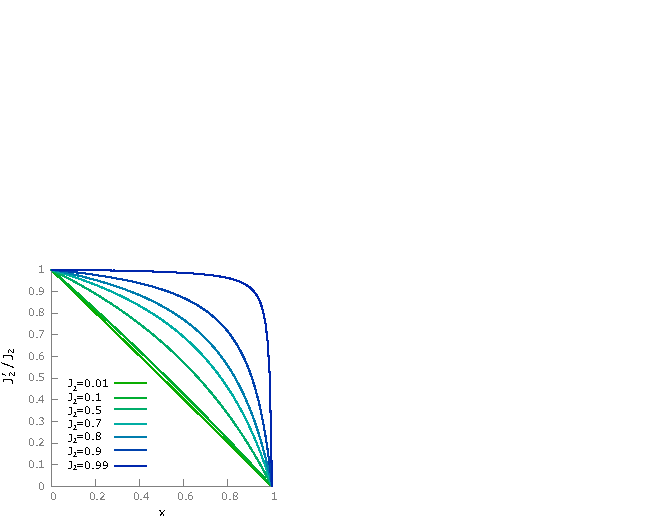
\includegraphics[width=.4\columnwidth,angle=0]{J2renorm.pdf}
%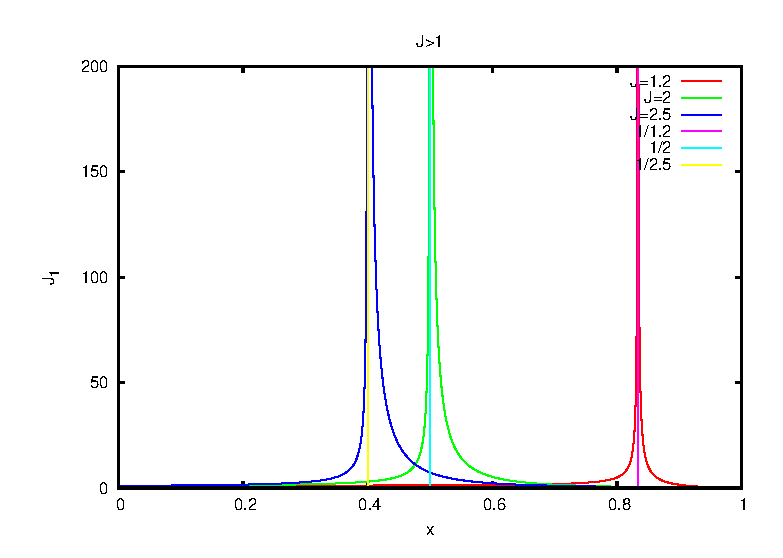
\includegraphics[width=.4\columnwidth,angle=0]{j_ordered.eps}
%\includegraphics[width=.6\columnwidth,angle=0]{jnew.eps}
\caption{We plot the effective interaction as function of the unobserved nodes $x$. On the left panel we show the behavior of 
the renormalized coupling $J_2/J$ for different values of $\beta J$. The closer to the critical point the less the hidden nodes affect
the interaction. While in the right panel we show the behavior of $-(1-x) J_4/J_2<1/3$. The 4-body interaction term is always smaller and negative with respect to the 2 body interaction term. The factor $1-x$ is added to compare dimensionless parameter $J_4$ with respect to the dimensionless parameter $J_2$.}
\label{fig:aboveTc}
\end{figure}

Below the critical temperature this analysis is still valid but we need to expand the saddle point solution (\ref{saddlemagn}) when a non vanishing zero solution appears. 

\subsection{Generalized calculation to four body interaction term}

In order to get the renormalization of the four body interaction term, we need to start from $J_2$ and $J_4$
\begin{eqnarray}
&&P(\{\sigma_i\},\{\tau_a\})=\frac{1}{Z} \exp\left( \frac{J_2}{2 N} \sum_{i  j} \sigma_i \sigma_j +\frac{J_4}{ 4N^3}\sum_{i j k l}  \sigma_i\sigma_j\sigma_k \sigma_l \right)\times\nonumber\\ &&\exp  \frac{J_2}{2 N} \left(2 \sum_{ia} \sigma_i \tau_a + \sum_{a b}\tau_a \tau_b \right)+ 
\frac{J_4}{4N^3 } \left( 4 \sum_{i j k a}  \sigma_i\sigma_j\sigma_k \tau_a + 6 \sum_{ijab} \sigma_i \sigma_j \tau_a\tau_b
+ 4 \sum_{iabc} \sigma_i \tau_a\tau_b\tau_c + \sum_{abcd} \tau_a\tau_b\tau_c\tau_d \right)
\end{eqnarray}
where we put $\beta=1$ and $J_4$ has to rescale $1/N^2$ in order to maintain the energy extensive.
In this case in presence of hidden variable $\tau_a$ there are higher order terms. Performing the 
partial sum constraining the hidden magnetization $m_h=1/(N x) \sum_a\tau_a$  is still possible when they are
fully connected and we get
\begin{eqnarray}
&&P(\{\sigma_i\},m_h)= \frac{1}{Z} \exp\left(\frac{ J_2}{2N}  \sum_{ij} \sigma_i \sigma_j + \frac{ J_4 }{4 N^3 } \sum_{ijkl} \sigma_i \sigma_j\sigma_k \sigma_l \right)\times \exp\left (Nx s(m_h)+ \frac{J_2 x }{2} \left( 2 \sum_i\sigma_i m_h + Nx m_h^2 \right)\right) \nonumber\\ && \exp\left(\frac{J_4 x}{4 N^2} \left( 4 \sum_{ijk} \sigma_i\sigma_j\sigma_k m_h + 6 N x \sum_{ij} \sigma_i \sigma_j m_h^2 + 4 (Nx)^2 \sum_i \sigma_i m_h^3 + (Nx)^3 m_h^4 \right)\right)
\end{eqnarray}
Before performing the saddle point approximation we can write the following hamiltonian as
\begin{equation}
P(m_o,m_h)=\sum_{\sigma_i} P(\{\sigma_i\},m_h) \delta(1/N(1-x) \sum_i \sigma_i-m_o)
\end{equation}
obtaining that
\begin{equation}
P(m_o,m_h)= \frac{1}{Z} \exp(-N_o f(m_o,m_h))
\end{equation}
where $N_o=N(1-x)$ and the density free energy reads
\begin{eqnarray}
f(m_o,m_h)&=&-\frac{J_2}{2} (1-x) m_o^2 - \frac{J_4}{4} (1-x)^3  m_o^4- s(m_o) - \frac{x}{1-x} s(m_h) + \frac{x}{1-x}e(m_h) \end{eqnarray}
with $$e(m_h)=- \frac{J_2 x}{2}  m_h^2- J_2 (1-x)m_o m_h - \frac{ 3 J_4 x (1-x)^2}{2 } m_o^2 m_h^2 -J_4 (1-x)^3 m_o^3 m_h 
- J_4 x^2 (1-x) m_o m_h^3 - \frac{J_4 x^3 }{4} m_h^4
$$
Performing the integral over $m_h$ can be still performed using the saddle point approximation obtaining the following equation
\begin{equation}
\hat{m}_h=\tanh\left(-e'(\hat{m}_h)\right)
\end{equation}
where $e'(m)=de(m)/dm$ is the first derivative. This allows to obtain the solution $\hat{m}_h(m_o)$ and performing an expansion in $m_o$ we get
$\hat{m}=a_1 m_o + a_2 m_o^2 +a_3 m_o^3+\ldots$
\begin{equation}
a_1=J_2 \frac{1-x}{1-J_2 x} \qquad a_3 = \frac{(x-1)^3 \left(J_2^3-3 J_4\right)}{3 (J_2 x-1)^4}
\end{equation}
Once obtain this expansion we can compute the free energy expansion $f(m_o,\hat{m})= -\frac{J'_2}{2} m_o^2 - \frac{J'_4 }{4}m_o^4 -s(m_o)$
such that
$$J'_2 =\frac{J_2 (1-x)}{1-J_2 x} \qquad J'_4= \frac{(x-1)^3 \left(J_2^4 x-3 J_4\right)}{3 (J_2 x-1)^4}$$ 

%Those can be identified through order by order expansion of (\ref{saddlemagn}) and we get that
%\begin{eqnarray}
%\overline{m}&=&\tanh( \beta J x \overline{m})\nonumber\\
%a_1&=&\frac{\beta  J \left( \overline{m}^2-1\right) (x-1)}{\beta  J x\left( \overline{m}^2-1\right) +1}\nonumber \\
%a_2 &=& \frac{\beta^2J^2 \overline{m} \left(\overline{m}^2-1\right) (x-1)^2}{\left(\beta J x \left(\overline{m}^2-1\right) +1\right)^3}\nonumber\\
%a_3 &=&-\frac{\beta ^3 J^3 \left(\overline{m}^2-1\right) (x-1)^3 \left(3 \beta  J x \overline{m}^4 -\overline{m}^2 (2 \beta  J x+3)-\beta  J x+1\right)}{3 \left(\beta  J x\left(\overline{m}^2-1\right) +1\right)^5}\nonumber\\
%%a_4 &=&\frac{\beta ^4 J^4 \overline{m} \left(\overline{m}^2-1\right) (x-1)^4 \left(3 \beta ^2 J^2 x^2 \overline{m}^6 +\overline{m}^2 \left(-3 \beta ^2 J^2 x^2+10 \beta  J x+3\right)+3 \beta ^2 J^2 x^2-3 \beta  J \overline{m}^4 x (\beta  J x+3)-\beta  J x-2\right)}{3 \left(\beta  J x\left(\overline{m}^2-1\right) +1\right)^7} \nonumber\\
%%a_5&=&-\frac{\beta ^5 J^5 \left(\overline{m}^2-1\right) (x-1)^5 \left(15 \beta ^3 J^3 \overline{m}^{10} x^3-15 \beta ^2 J^2 \overline{m}^8 x^2 (\beta  J x+6)+6 \beta  J \overline{m}^6 x \left(-7 \beta ^2 J^2 x^2+25 \beta  J x+15\right)+\overline{m}^4 \left(66 \beta ^3 J^3 x^3-26 \beta ^2 J^2 x^2-135 \beta  J x-15\right)+\overline{m}^2 \left(-21 \beta ^3 J^3 x^3-38 \beta ^2 J^2 x^2+44 \beta  J x+15\right)-(\beta  J x-1)^2 (3 \beta  J x+2)\right)}{15 \left(\beta  J x\left(\overline{m}^2-1\right) +1\right)^9}\nonumber
%\end{eqnarray}
%After that we can identify all the interaction terms order by order by obtaining the saddle point equation. 
%This is due to the fact that once you have a general energy
%density function $e(m_o)=-h m_o - J_2 m_o^2/2 - J_3 m_0^3/3 + \ldots$ we get a self consistent equation of the following type 
%\begin{equation}\label{jkdef}
%m_o=\tanh( \beta h + \beta J_2 m_o + \beta J_3 m_o^3 + \beta J_4 m_o^4 +\ldots)
%\end{equation}
%where we can identify all the $J_k$ with the term in the expansion.
%
%So now let us obtain the self consistent equation for $m_o$ in order to identify all the interaction terms. 
%We should derive the free energy with respect to $m_o$, $\partial_{m_o} f(\hat{m},m_o)=0$.  In particular in our case since $\hat{m}$ is a function of $m_o$ itself and given equation (\ref{saddlemagn}), we obtain 
%\begin{equation}
%\partial_{m_o} \hat{m} = \frac{ \sqrt{1-\hat{m}^2} }{ 1 - \beta J x  \sqrt{1-\hat{m}^2}}\beta J (1-x)
%\end{equation} 
%Then by using the effective energy (\ref{energy}) and expanding in series of $\hat{m}$ we get that
%\begin{eqnarray}
%m_o= \tanh\left(\beta J (1-x) m_o + \beta J x \hat{m} - \frac{\beta J x }{2(\beta J x -1)}\hat{m}^3 + o(\hat{m}^5)\right) 
%\end{eqnarray}
%Since $\hat{m}=  a_1 m_o  + a_3 m_o^3 + \ldots $, we get that the self consistent equation reads
%$$ m_o=\tanh\left( \beta J ( 1-x + x a_1 ) m_o + \beta J x \left(a_3- \frac{a_1^3}{2 (\beta J x -1)}\right) m_o^3 + \ldots \right)\,.$$ As showed by equation (\ref{jkdef}), we are thus able to identify the new coupling $J_k$ in terms of the parameters $a_i$'s.
%Whenever $\beta J <1$, there will be only one solution around zero $\overline{m}=0$ namely the hidden system is disordered, so $\hat{m}$ is an odd function of $m_o$ such that the things simplify
%\begin{eqnarray}\label{renJ1hT}
%J_2&=&  J(1-x + x a_1)\nonumber\\
%J_4&=& J x \left(a_3- \frac{a_1^3}{2 (\beta J x -1)}\right)
%\end{eqnarray}
%and given the parameters we obtain that the renormalized interactions read 
%\begin{eqnarray}
%a_1&=& \frac{\beta  J (1-x)}{1-\beta  J x} \;\Rightarrow \; J_2=\frac{J(1-x)}{1-\beta J x}\nonumber \\
%a_2 &=& 0 \nonumber\\
%a_3 &=& -\frac{\beta ^3 J^3 (1-x)^3}{3 (1-\beta  J x)^4} \;\Rightarrow \; J_4 =\frac{\beta^3 J^4 (1-x)^3 x}{6(1-\beta J x)^4}\nonumber\\
%a_4 &=& 0\nonumber\\
%%a_5&=&\frac{\beta ^5 J^5 (x-1)^5 (3 \beta  J x+2)}{15 (\beta  J x-1)^7}
%\end{eqnarray}
%recovering the result above the critical temperature and obtaining before.

%Below critical temperature $\beta J>1$ we need to distinguish two cases: 
%\begin{itemize}
%\item above the hidden system critical temperature $\beta J x<1$. This means that $x<1/\beta J$ that is in the range below the unity  and also $(1-\beta J x )>0$. In this regime, $\overline{m}=0$ so that the parity of the free energy is recovered $J_1=J_3=J_5=0$.
%The system is thus not stable and diverge to infinity at a critical value $x_c=1/\beta J$. This is due to the fact that the system developed a long range correlation so the renormalization procedure
%flows to strong coupling. The interactions are as above the critical temperature
%\begin{eqnarray}
%J_2= \frac{J (1-x)}{1-\beta  J x} 
%\end{eqnarray}
%In this regime the denominator of $J_2$ diverge at the critical value $x_c=(\beta J)^{-1}$. The system exhibits a strong coupling behavior meaning that the variables get strongly coupled. 
%\item below the hidden system critical temperature $\beta J x >1$. We should consider the onset of a non null magnetization $\overline{m}$ that behaves as an external magnetic field. This makes calculation more complicated but we can expand oder 
%by order when $\overline{m}$ is small meaning when $\beta J x \approx 1$. 
%We thus obtain $J_2/J$ and $J_4/J_2$ and show their 
%The analytic solution for 
%$\overline{m}\approx \sqrt{3(\beta J x-1)/(\beta J x)^3}$ giving that $J_2$ reads
%%\begin{equation}
%%\frac{J_2}{J}=\frac{4 (\beta J x)^4 (x-1) }{4 (\beta J x)^5 + \sqrt{-5 (\beta J x)^5 (19 \beta J x-24)}-4 (\beta J x)^4-5 (\beta J x)^3}
%%\end{equation}
%\end{itemize}
%\begin{figure}
%\includegraphics[width=.7\columnwidth,angle=0]{}
%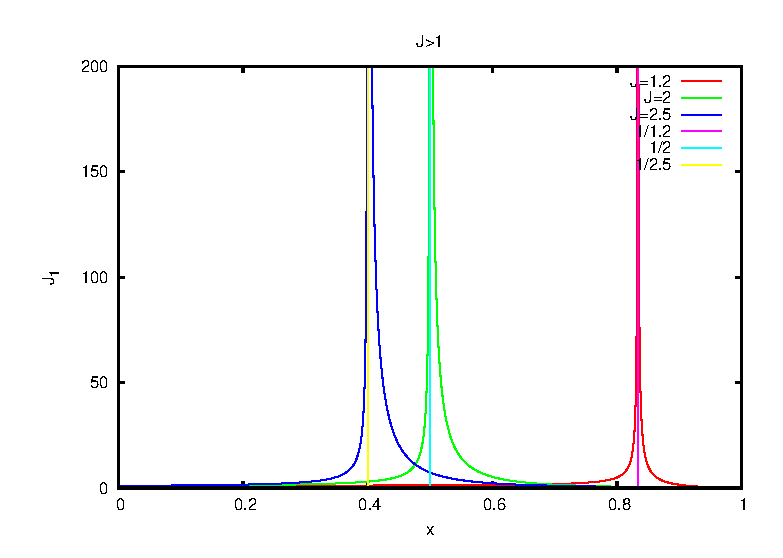
\includegraphics[width=.4\columnwidth,angle=0]{j_ordered.eps}
%\includegraphics[width=.6\columnwidth,angle=0]{jnew.eps}
%\caption{We plot the effective interaction as function of the unobserved nodes $x$ around $\beta J x \approx 1 $. On the left panel we show the behavior of 
%the renormalized coupling $J_2/J$ for different values of $\beta J$ below the critical temperature $\beta J > 1$ while
%on the left the value of $J_4/J_2.$}
%\label{fig:belowTc}
%\end{figure}



% We plot those adimensional parameters in figure \ref{fig:aboveTc} and \ref{jrenorm} where $J_4$ is going to zero much faster than $J_2$ around the critical values.
%\begin{figure}[h]
%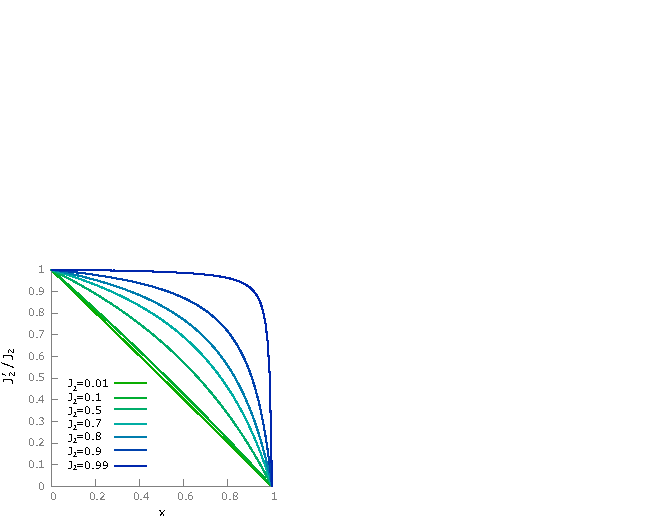
\includegraphics[width=.49\columnwidth]{J2renorm.pdf}
%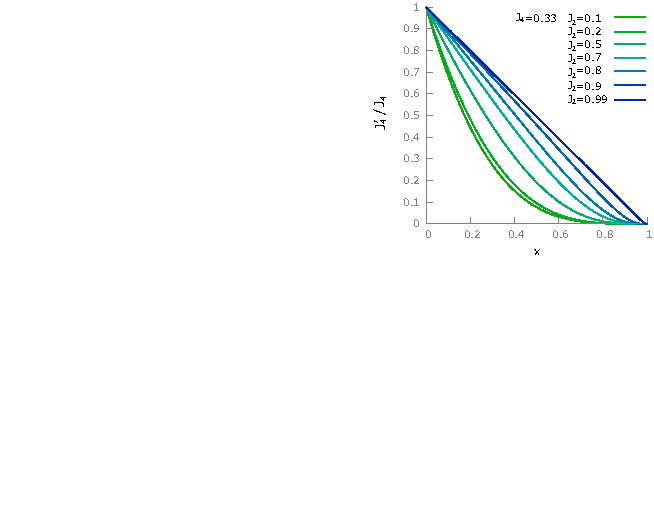
\includegraphics[width=.49\columnwidth]{J4_j2.pdf}
%\caption{In left figure we plot how the adimensional coupling constants get renormalized. }
%\label{jrenorm}
%\end{figure} 
\begin{figure}[h]
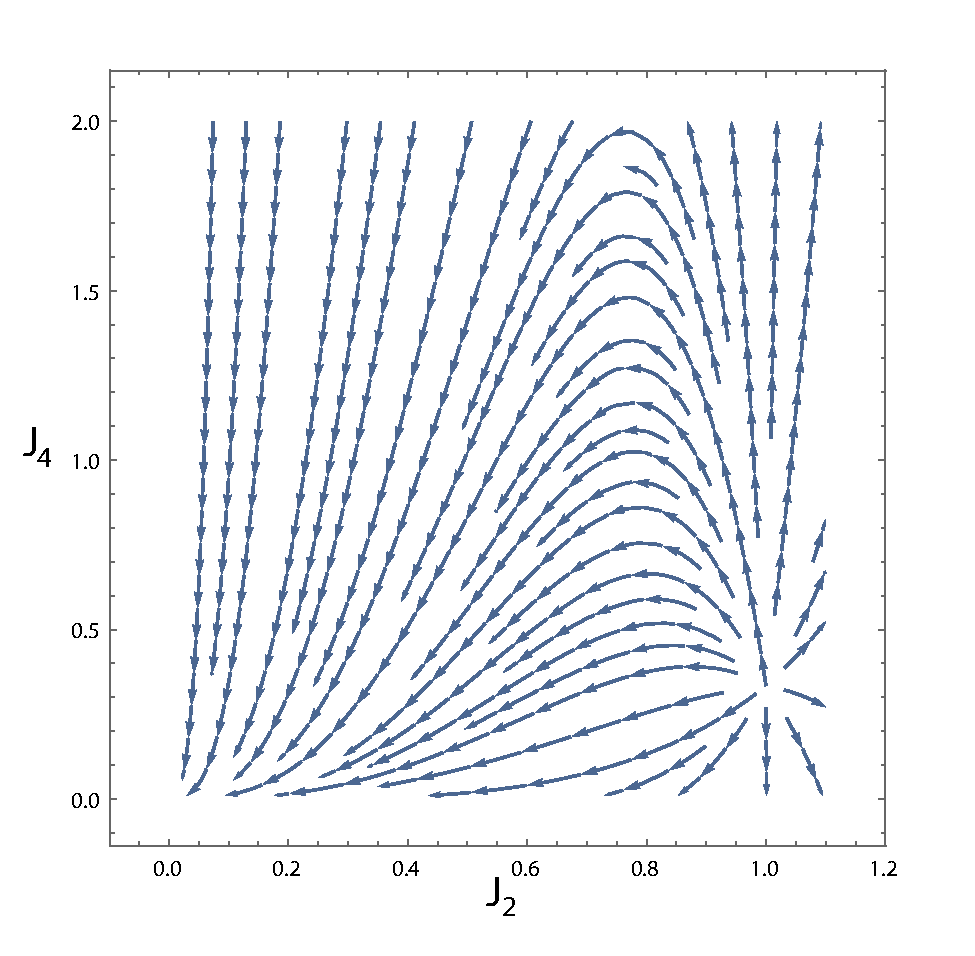
\includegraphics[width=.5\columnwidth]{beta_lines.pdf}
\caption{In figure we plot the renormalization flux valid whenever $J_4>J_2^3/3$ otherwise the solution only solution for the magnetization is zero. The fixed point $\beta J_2=1$ $\beta J_4=1/3$ is an unstable fixed point while the stable fixed point is the trivial one.}
\label{beta functions}
\end{figure} 
Those equations show one non trivial fixed point $ J_2=1, J_4=1/3$ apart from the trivial one $J_2=0, J_4=0$. 
Once we obtain the renormalized couplings we can check the behavior around the non trivial fixed point when we let $b=1/(1-x)\to \infty$. This is obtained by the linear correction
$$\left.\frac{ \delta J'_2}{\delta J_2} \right |_{J_2^*}=b \quad \left.\frac{ \delta J'_2}{\delta J_4} \right |_{J_2^*}=0 \quad \left.\frac{ \delta J'_4}{\delta J_2} \right |_{J_2^*,J_4^*}=0 \quad \left.\frac{ \delta J'_4}{\delta J_4} \right |_{J_2^*,J_4^*}= b$$
We see that the linear correction increase with increasing $b\to \infty$ showing a coefficient $\mu =1$, both couplings are relevant operators around the non-trivial fixed point.
Differently around zero they are both irrelevant operator but $J_4$ has a exponent that is much higher. So it goes to zero faster than $J_2$ and can be neglected.
Moreover we can write explicitly the beta function whose flux is shown in Figure \ref{beta functions}
\begin{equation}\label{eq1:flux}
\beta_2(J_2) = b \frac{\partial \log J_2}{\partial b}= (1-x) \frac{\partial \log J_2}{\partial x} = \beta J_2 -1
\end{equation}
so we get a fixed point $\beta J_2=1$. In the same way we get the four body interaction term
\begin{equation}
\beta_4(J_2, J_4) = (1-x) \frac{\partial \log J_4}{\partial x} =\frac{J_2^5 x^2+J_2^4 (1-2 x)-3 J_2 J_4+3 J_4}{(J_2 x-1) \left(J_2^4 x-3 J_4 \right)}\end{equation}
In terms of the coupling constants we obtain 
\begin{equation}\label{eq2:flux}
\beta_4(J_2, J_4)  =    3 (\beta J_2 -1)+ \beta J_2\left(1-\frac{(\beta J_2)^3}{3\beta J_4} \right) 
\end{equation}
Those equations can be linearized in term of the fixed point $\beta J_2^*=1$ and $\beta J_4^*=\frac{1}{3}$ such that $M_{ij}=\partial J_i/\partial J_j$
where $M_{22}=1$, $M_{24}=0$, $M_{42}=6$ and $M_{44}=-3$. By computing the eigenvalues we get the dimension of the two couplings:  $J_2 \propto b$ while $J_4\propto b^-3$, this means that $J_2$ is a relevant operator while $J_4$ has a negative dimension so that is an irrelevant one.

Perform an inference method and obtain $J$ out of the correlation for different observed degrees of freedom $x$. This will show how close to the critical point you may be.
Moroever how this is affected by $M/N$?

 %Instead for the last coupling constant $J^a_6$ 
%\begin{equation}
%\beta_6(J^a_2, J^a_4,J^a_6) = 4+ (1-\beta J'_2) \left(5 + \frac{6}{5} \frac{(\beta J^a_4)^2}{\beta J^a_6 (\beta J^a_2)^2}\right)- 2\beta J^a_2 \left( 1+ \frac{1}{15} \frac{(\beta J^a_2)^5}{ \beta J^a_6} - \frac{3}{5}  \frac{(\beta J^a_2)^2 \beta J^a_4}{\beta J^a_6}\right) 
%\end{equation}

\subsection{Natural Dimension, beta functions and relevant operators}

Let us discuss their dimensions as function of the renormalization parameter $b=1/(1-x)$. We know that above the critical temperature
we can define the new block variable $\sigma_o=1/(b^{\omega}) \sum_{i=1}^{b} \sigma_i $. Since we have the gaussian fix point  where every variable is independent with null mean value and fixed variance $\Delta$, we have that $$\langle \sigma_o^2\rangle = b^{1-2 \omega} \langle \sigma^2\rangle $$ So that the dimension of the magnetization is $\omega=1/2$. In this regime when integrating over $b=1/(1-x)$ degrees of freedom we thus get that $m_o \to m_o \sqrt{b}$. After rescaling $N \to N'= N /b$, so in order to keep the energy extensive  we have that each interactions get a renormalization factor due to its natural dimension
$$J_2 \to J_2  \qquad J_4 \to  J_4 b \qquad J_6 \to J_6 b^2\,.$$
In this case since $b=1/(1-x)$ we get that the adimensional running coupling constant $$J^a_2=J_2 \qquad J^a_4=J_4 / b=J_4 (1-x) \qquad J^a_6=J_6 /b^2=J_6(1-x)^2$$

\section{Small $x$ expansion}

In the general case where we don't know the initial energy function $e(m)$ the calculation can be done in full generality obtaining the renormalized
form $e'(m)$ by an expansion with respect to $x$ namely the fraction of nodes that we integrate out. 
Suppose that we have the intensive order parameter $m$, we can write in full generality that the probability of a given configuration is
\begin{equation}
P(m)=\frac{1}{Z} e^{- N \big(e(m) - s(m)\big)}
\end{equation}
If we introduce $m'$ and $m_o$ such that $m=m_o + x(m'-m_o)$ and assuming the entropy is additive we also have that
 $$s(m) = (1-x) s(m_o) + x s(m')\,.$$
Let us introduce the probability function of the observed systems by integrating out over the unobserved degrees of freedom 
$$P(m_o)=  \frac{1}{Z} e^{N(1-x) s(m_o) }\int dm' e ^{-N \big( e( m_o + x(m'-m_o)) - x s(m')\big)}$$
Now performing an expansion in$x$ of the energy function we get
$$P(m_o)=  \frac{1}{Z} e^{N(1-x) s(m_o) -N e(m_o) }\int dm' e ^{ N x s(m') -N x (m'-mo) e'( m_o)  - N \frac{x}{2} (m'-mo)^2 e''(m_o) + O(x^2)}$$
where $e'(m_0)=de(m)/dm|_{m_o}$ and $e''(m_0)=d^2e(m)/dm^2|_{m_o}$. By a saddle point approximation we get that the optimal $m'$ satisfy this 
equation 
\begin{equation}\label{saddlepoint}
s'(\hat{m}) = e'(m_o) + x(\hat{m}-m_o) e''(m_o)\,.
\end{equation}
If we define the new energy and entropy $P(m_o) \propto e^{N_o s(m_o) - N_o e(m_o) }$ we get that
$$(1-x) s(m_o) - e(m_o) + x \left[ s(\hat{m}) - (\hat{m}-m_o) e'(m_o) - \frac{x}{2} (\hat{m}-m_o)^2 e''(m_o)\right] $$
Knowing the entropy function $$s(m)=-\frac{1-m}{2} \log\frac{1-m}{2} -\frac{1+m}{2} \log\frac{1+m}{2}=-\frac{1}{2} \log \frac{1-m^2}{4} + m s'(m)$$
we get that $s(\hat{m})= \hat{m} e'(m_o) + x \hat{m} (\hat{m}-m_o) e''(m_o) -\frac{1}{2} \log \frac{1-\hat{m}^2}{4}$. Using this expression into the previous equation we get that
\begin{eqnarray}
&&(1-x) s(m_o) - e(m_o) + x \left[ \hat{m} e'(m_o)  + x \hat{m} (\hat{m}-m_o) e''(m_o) - (\hat{m}-m_o) e'(m_o) - \frac{x}{2} (\hat{m}-m_o)^2 e''(m_o) -\frac{1}{2} \log \frac{1-\hat{m}^2}{4}\right] \nonumber\\
&&(1-x) s(m_o) - e(m_o) + x \left[ m_o e'(m_o)  - \frac{x}{2} m_o^2 e''(m_o)  + \frac{x}{2} \hat{m}^2 e''(m_o)-\frac{1}{2} \log \frac{1-\hat{m}^2}{4}\right]  \nonumber\\
&&(1-x) s(m_o) - e((1-x) m_o)  + \frac{x^2}{2} \hat{m} e''(m_o)-\frac{x}{2} \log \frac{1-\hat{m}^2}{4}
\end{eqnarray}
So we see that the entropy part is not modified but the energetic contribution get renormalized by the integrated variable such that
$$ e(m) \to \frac{1}{1-x} \left(e((1-x) m_o)  - \frac{x^2}{2} \hat{m} e''(m_o) + \frac{x}{2} \log \frac{1-\hat{m}^2}{4}\right)$$
with $\hat{m}=\tanh ( - e'(m_o)-x (\hat{m}-m_o) e''(m_o)) )$ given the self consistent equation (\ref{saddlepoint}) and $s'(m)=-\mbox{atanh}(m)$.
Here we have to expand order by order in $x$ obtaining at the end $de(m)/dx$.

Let us start with $\hat{m}=-\tanh(e'(m_o) + x (\hat{m}-m_o) e''(m_o))$. Here we get up to first order since this term is multiplied by $x^2$
\begin{equation}
\hat{m}= -\tanh(e'(m_o)) - x (\hat{m}-m_o) e''(m_o) (1-\tanh^2(e'(m_o))) + o(x^2)
\end{equation} 
and consequently
\begin{equation}
\log \frac{1-\hat{m}^2}{4}= \log\frac{1-\tanh^2(e'(m_o))}{4} - 2 x (\hat{m}-m_o) e''(m_o) \tanh(e'(m_o)) + o(x^2)
\end{equation} 
Using the previous results we get that
\begin{eqnarray}
e(m_o) &\to& \frac{e((1-x) m_o)}{1-x}  + \frac{x^2}{2} \hat{m} e''(m_o)-\frac{x}{2} \log \frac{1-\hat{m}^2}{4} +O(x^2)\nonumber\\
&\to& e(m_o) (1+x) - x m_o e'(m_o)  + \frac{x^2}{2}e''(m_o) \tanh^2(e'(m_o)) -\frac{x}{2}  \log\frac{1-\tanh^2(e'(m_o))}{4} \nonumber \\ && \hspace{3cm} + x^2 (\hat{m}-m_o) e''(m_o) \tanh(e'(m_o)) + O(x^2)\nonumber\\
&\to&  e(m_o) + x \left[e(m_o) - m_o e'(m_o) + \log \frac{1-\tanh^2(e'(m_o))}{4}\right] +O(x^2)
\end{eqnarray}
Finally we obtain that the first order correction of the energy is the following
\begin{equation}\label{eq:energyrenormalization}
\frac{de}{dx}= -m_o e'(m_o) + e(m_o) +\frac{1}{2} \log \frac{1-\tanh^2(e'(m_o))}{4}
\end{equation}

\begin{itemize}
\item natural dimension $N f(m) = \phi(N^\alpha m)=$ fixed. Depends how the field rescales
\item k-space RG PCA.
\end{itemize}


\textbf{Some applications} 
\begin{itemize}
\item \textit{Two body interaction term}

Let us see if we obtain the same results that we obtain before by assuming that
$e(m)=-1/2 J m^2$ and $e'(m)=-J m$ we get that for $m\ll 1$. From equation (\ref{eq:energyrenormalization}) we get 
\begin{equation}
\frac{1}{J}\frac{dJ}{dx}= J-1
\end{equation}
This is the same result reported in equation (\ref{eq1:flux}) since the sign comes from the
small $x$ expansion 
$$(1-x) \frac{d\log J}{d x} \sim   \frac{d\log J}{dx}$$
where the approximation is true whenever $x$ is small.
So whenever $J<1$ that is consistent with $m\ll 1$, decimation is reducing the renormalized interaction strength leading to weak coupling regime.
We get that $J \to 0$ when we decimate apart for $J=1$ that is a fixed point of the dynamics.
This expansion is valid also when $J>1$ because it assumes only that the magnetization is small. 
This is the case around the fixed point where $m\sim \sqrt{J-1}$. We found a way to see relevant and irrelevant parameters throughout the computation of their renormalization with respect to integration of the hidden variables.

\item \textit{Four body interaction term}

In presence of a 4-body interaction term $e(m)= -J_2/2 m^2-J_4/4 m^4$ we get
$$\frac{1}{J_2}\frac{dJ_2}{dx}= J_2-1 \qquad \frac{1}{J_4} \frac{dJ_4}{dx}= 3(J_2-1) + J_2(1-\frac{J_2^3}{3 J_4})$$
and as before it is in agreement with the previous results in equation (\ref{eq1:flux}) and (\ref{eq2:flux}). \end{itemize}
\end{document}